\chapter{Introduction}

Over three million published articles on pubmed with keyword \textit{cancer} shows the huge amount of research effort for understanding, diagnosing and treating cancer diseases. The research focus is mainly on tumor cells, but a segment of interest which is increasing is research on tumor stroma as seen in figure \ref{fig:pubmed}. Tumor stroma is basically the environment of cells that is suppressing or supporting the function of the tumor cells. It is suggested that under the development of a tumor, the stroma is changing from being suppressive to supportive of the tumor cells.

\begin{figure}[h]
\centering
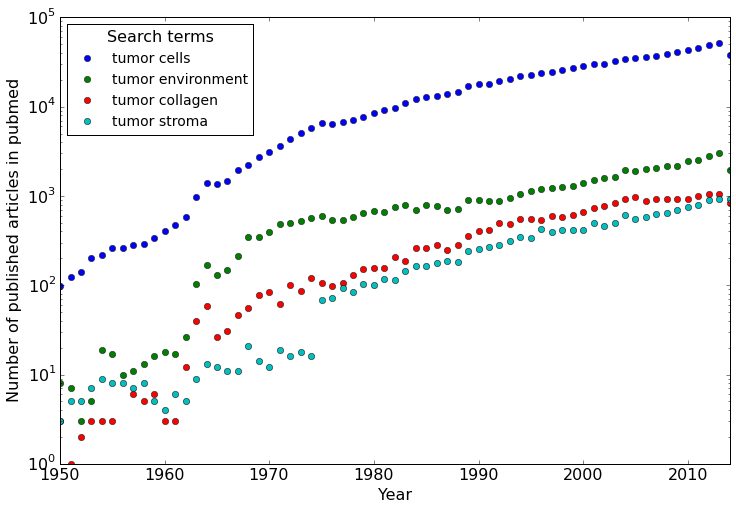
\includegraphics[width=10cm]{pubmed_tumor}
\caption{Amount of published articles by year on different search terms. The search term \textit{tumor cells} outnumber the others by two orders of magnitude. Note the logarithmic scale on y-axis.}
\label{fig:pubmed}
\end{figure}

In particular, collagen fiber is known to be altered in the surroundings of tumor cells under the development towards metastasis. One bio-marker for collagen fibers, is their alignment at the vincinity of the tumor, which may predict if a tumor is malignant. The fiber alignment can be used as a diagnosis tool for malignant tumor, and an article written at NTNU have studied collagen fiber alignment in a manual qualitative manner \cite{anna}.

St. Olav hospital have taken breast tissue samples from 900 pasients. In total three samples per patient, one sample inside, one sample at the boundary and one sample outside the tumor. The samples is laid in a matrix on a glass slide, each glass slide having about 130 samples. As microscope scanning and analysis of such a large data set is not straightforward, this project have explored possibilities for automating the process.

To be specific, the goals of the project were:
\begin{itemize}
\item  Find good parameters for obtaining high quality images
\item Find an effective way to scan whole glass slides of 135 samples with little human intervention
\item Store the images in a structured manner so that 
    \begin{itemize}
    \item Correlation to patient data is possible
    \item Quantitative data can be subtracted
    \end{itemize}
\item Try some algorithms for creating quantitative data
\end{itemize}